\chapter{Introducción}

La inteligencia artificial (\acrshort{ia}) se ha posicionado como uno de los pilares fundamentales de la innovación tecnológica y el desarrollo en el siglo XXI, marcando un antes y un después en la forma en que interactuamos con nuestro entorno y concebimos el futuro. Esta disciplina, que abarca desde el aprendizaje automático hasta la robótica y el procesamiento del lenguaje natural, ofrece promesas sin precedentes para el avance de la ciencia, la mejora de la calidad de vida y la optimización de procesos en prácticamente todos los sectores de la actividad humana. Sin embargo, su rápida evolución también plantea interrogantes críticos sobre ética, seguridad, privacidad y la dinámica del empleo, desafíos que esta investigación se propone explorar.

\section{Contexto y Motivación}

La inteligencia artificial, en su búsqueda por emular la capacidad cognitiva humana, ha evolucionado de simples \glspl{algoritmo} a sistemas capaces de aprender y adaptarse. Esta sección delinea el contexto histórico, la motivación para su estudio intensivo y su papel transformador en la sociedad contemporánea. Como ejemplo, en la \autoref{fig:ai-future} se presenta una visión futurista de una ciudad avanzada, caracterizada por el uso integral de la inteligencia artificial.

\begin{itemize}
    \item Evolución histórica de la \acrshort{ia}: Un recorrido desde sus conceptos teóricos iniciales hasta las implementaciones avanzadas de hoy en día.
    \item Innovaciones tecnológicas fundamentales: Descripción de los avances en aprendizaje profundo, visión por computadora y sistemas autónomos.
    \item Transformación sectorial: Análisis de cómo la \acrshort{ia} está redefiniendo la medicina, la educación, la industria financiera y el entretenimiento digital.
    \item Impacto social: Consideración de las implicaciones de la \acrshort{ia} en la privacidad, el empleo y la ética.
\end{itemize}

\begin{figure}[ht!]
	\centering
	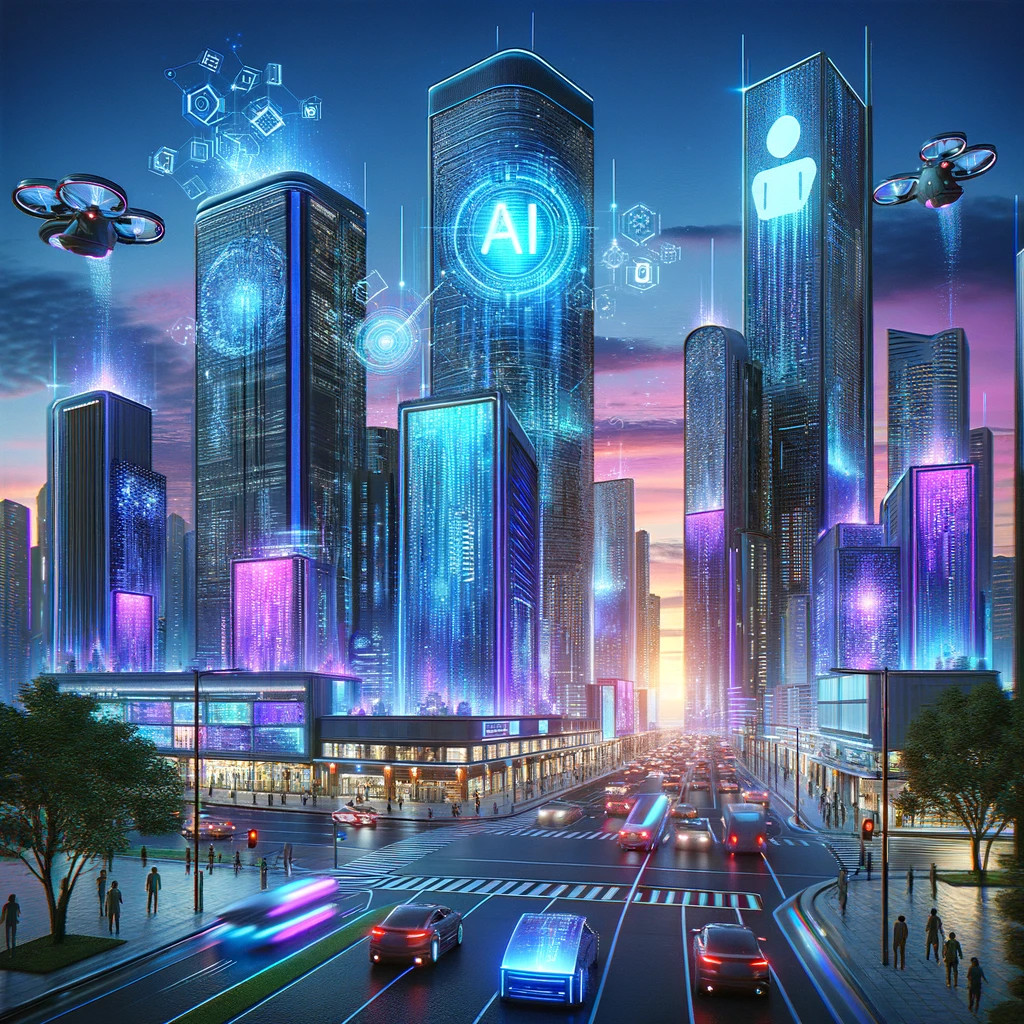
\includegraphics[width=0.75\textwidth]{chapters/1_introduction/figures/image_ia.jpg}
	\caption{\textbf{El futuro con IA.} Esta imagen presenta un panorama futurista de una ciudad avanzada, caracterizada por el uso integral de la inteligencia artificial. Destacan vehículos autónomos volando entre rascacielos que exhiben \glspl{algoritmo} de IA y códigos digitales en sus fachadas iluminadas con neón. El cielo, en tonos púrpuras y azules, refleja la fusión de tecnología y vida diaria, mientras las personas interactúan con interfaces holográficas. Esta visión sugiere un futuro donde la IA mejora la conectividad y eficiencia urbana, subrayando el impacto transformador de la tecnología en nuestra sociedad.}
	\label{fig:ai-future}
\end{figure}

\section{Problema de Investigación}

La adopción generalizada de la \acrshort{ia} viene acompañada de una serie de desafíos éticos y técnicos. Este estudio se centra en identificar y proponer soluciones a los problemas que surgen con la implementación de sistemas de \acrshort{ia}, incluyendo sesgos algorítmicos, seguridad de los datos y la brecha digital.

\subsection{Objetivos de la Investigación}

\begin{enumerate}
    \item Investigar las tendencias actuales en el desarrollo de la inteligencia artificial y su aplicación en campos clave.
    \item Examinar los desafíos éticos, legales y sociales emergentes asociados con la proliferación de la \acrshort{ia}.
    \item Desarrollar un conjunto de principios y recomendaciones para guiar el desarrollo ético y responsable de la \acrshort{ia}.
    \item Evaluar el impacto de la \acrshort{ia} en la dinámica del mercado laboral y proponer estrategias para la adaptación y capacitación.
\end{enumerate}

\section{Justificación y Contribuciones}

La importancia de este trabajo reside en su enfoque multidisciplinario para comprender la inteligencia artificial, no solo desde una perspectiva técnica sino también considerando sus ramificaciones éticas y sociales.

\begin{itemize}
    \item Ampliación del conocimiento académico: Este estudio contribuye a la literatura existente ofreciendo un análisis profundo de la intersección entre la \acrshort{ia} y áreas críticas de la vida humana.
    \item Diálogo ético y social: Fomenta una discusión necesaria sobre cómo la humanidad debe navegar los avances en \acrshort{ia}, promoviendo un desarrollo tecnológico que respete los valores humanos fundamentales.
    \item Guía para la acción: Proporciona recomendaciones prácticas para desarrolladores, legisladores y la sociedad en general, sobre cómo abordar los desafíos presentados por la \acrshort{ia} de manera proactiva y positiva.
\end{itemize}

\section{Contribuciones al Conocimiento y la Sociedad}

Este trabajo aspira a ser un recurso valioso para comprender mejor los complejos desafíos que presenta la inteligencia artificial. A través de una exploración detallada de sus aplicaciones y las cuestiones éticas que suscita, se busca ofrecer una visión equilibrada que reconozca tanto los beneficios como los riesgos de la \acrshort{ia}. Al hacerlo, esta investigación apunta a:

\begin{itemize}
    \item Enriquecer el diálogo académico y público sobre la \acrshort{ia}, promoviendo una comprensión más matizada de su papel en la sociedad.
    \item Servir como base para el desarrollo de políticas públicas y estrategias empresariales que maximicen el potencial positivo de la \acrshort{ia} mientras se minimizan sus riesgos.
    \item Inspirar futuras investigaciones que continúen explorando la evolución de la inteligencia artificial y su impacto en diversas esferas de la vida humana.
\end{itemize}

Con un enfoque en la investigación interdisciplinaria, este estudio no solo aborda los aspectos técnicos de la \acrshort{ia}, sino que también se sumerge en las preguntas filosóficas, éticas y sociales que surgen de su integración en nuestra vida diaria. Se espera que los resultados de esta investigación iluminen el camino hacia un futuro en el que la tecnología y la humanidad coexistan en armonía, guiados por principios de equidad, inclusión y respeto mutuo.
